\chapter{Point de vue developpeur}

\section{Documentation}
qsdqsd
\clearpage
\section{Conception}
\subsection{Architecture}
Dans cette partie nous détaillerons l'architecture de notre application, à travers ses différents points d'extensions.
\begin{figure}[!htbp]
  \centering
  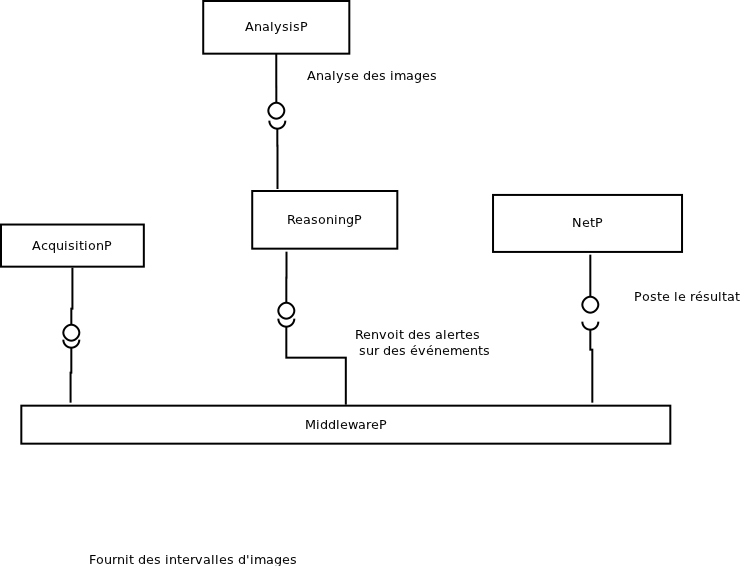
\includegraphics[scale=0.50]{img/archi}
  \caption{Architecture de l'outil}
  \label{fig:archi}
\end{figure}

\subsection{Classes}
dsqdqs
\paragraph{Architecture}
qsdqs
\paragraph{Acquisition}
Le plugin Acquisition consiste à récupérer un fichier vidéo et en extraire une image périodiquement. Le plugin répond aux spécifications fournies par l'interface \verb+IFlux+ (cf. Fig \ref{fig:IFlux}).
\begin{figure}[htbp]
  \centering
  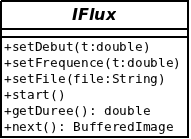
\includegraphics[scale=0.50]{img/IFlux}
  \caption{Interface IFlux}
  \label{fig:IFlux}
\end{figure}

Pour pouvoir lancer le plugin il est nécessaire d'appeler au minimum les méthodes suivantes dans cet ordre :
\begin{enumerate}
\item{\verb+setFile(file)+} pour fournir le fichier vidéo à analyser.
\item{\verb+start()+} Cette méthode permet de paramètrer l'aquisition et de charger un player. 
\item{\verb+next()+} renvoie un \verb+BufferedImage+ et avance dans la vidéo.
\end{enumerate}

Les autres méthodes de l'interface IFlux sont :
\begin{itemize}
\item{\verb+setDebut(tEnSecondes)+} pour donner l'instant à partir duquel la vidéo sera analysée. Cette méthode doit être lancée avant \verb+start()+ ou alors \verb+start+ est relancée
\item{\verb+setFrequence(tEnSecondes)+} Le nom de la méthode est trompeuse mais elle permet de donner la période en secondes à laquelle le plugin récupère un image dans la vidéo. La période peut être changée avant ou en cours d'acquisition. Cependant le pointeur sur la prochaine image à acquérir étant déjà défini, le changement de période ne sera effectif qu'à partir du second \verb+next()+
\item{\verb+getDurée()+} renvoie un le temps en secondes de la vidéo. \verb+start()+ doit avoir été déja lancée.
\end{itemize}

Pour effectuer l'acquisition le plugin utilise la librairie JMF qui est malheureusement peu pratique puisqu'elle ne gère qu'un faible nombre de formats vidéo. De plus nous avons pu constater un bug au niveau de la méthode qui renvoie la durée de la vidéo \verb+Player.duration()+; en effet celle-ci renvoie une valeur bien trop grande par rapport à la longueur réelle de la vidéo.

\paragraph{Reasoning}
sdqsd
\paragraph{NetP}
Le  NetP est dédié à poster des informations sur un  réseau social ou un blog. Un contributeur de ce point d'extension doit être en mesure de proposer une solution pour chaque action que recquière Middleware. Ces actions sont données dans l'interface \verb+IIformation+ suivante :
\begin{figure}[!htbp]
  \centering
  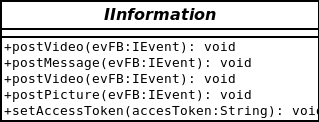
\includegraphics[scale=0.50]{img/iinterface}
  \caption{Interface pour NetP}
  \label{fig:IInterface}
\end{figure}

Le contributeur que nous avons implémenté propose d'utiliser le réseau social Facebook et utilise la librairie suivante \cite{restFB}.


\section{Robustesse}
sqdqs
\section{Qualité du code}
dqsdqs
\section{Facilité de mise en oeuvre des extension}
